\documentclass[sigplan]{acmart}

%New command for paragraphs
\newcommand{\adparagraph}[1]{\paragraph{#1}\mbox{}\\\noindent}

%Command for Markov chain 4
\usepackage{xspace}
\newcommand{\MC}{$\text{MC}_4$\xspace}

%Fixes the style of the ACM article template 
\settopmatter{printacmref=false} % Removes citation information below abstract
\renewcommand\footnotetextcopyrightpermission[1]{} % removes footnote with conference information in first column
\pagestyle{plain} % removes running headers

%Graph packages
\usepackage{tikz}
\usepackage{pgfplots}

%appendix setup
\usepackage{booktabs} % For formal tables
\usepackage[titletoc,toc,title]{appendix}

%note setup
\usepackage{xargs} 
\usepackage{xcolor}
\usepackage[colorinlistoftodos,prependcaption,textsize=tiny]{todonotes}
\newcommandx{\note}[2][1=]{\todo[linecolor=red,backgroundcolor=red!25,bordercolor=red,#1]{#2}\xspace}


% Copyright
\setcopyright{none}
%\setcopyright{acmcopyright}
%\setcopyright{acmlicensed}
%\setcopyright{rightsretained}
%\setcopyright{usgov}
%\setcopyright{usgovmixed}
%\setcopyright{cagov}
%\setcopyright{cagovmixed}
\usepackage{lineno}


\begin{document}
\linenumbers
\title{Group Recommendation}
%\titlenote{Produces the permission block, and copyright information}
\subtitle{Using Information Retrieval Rank Aggregation Methods}
%\subtitlenote{The full version of the author's guide is available as \texttt{acmart.pdf} document}

\author{Lasse Drustrup Christensen}
%\authornote{}
\affiliation{%
  \institution{Department of Computer Science Aalborg University}
  \streetaddress{Selma Lagerl\"{o}fs Vej 300}
  \city{Aalborg East} 
  \state{Denmark} 
  \postcode{9220}
}
\email{ldch11@student.aau.dk}

\author{Lukas Nic Dalgaard}
%\authornote{}
%\orcid{}
\affiliation{%
  \institution{Department of Computer Science Aalborg University}
  \streetaddress{Selma Lagerl\"{o}fs Vej 300}
  \city{Aalborg East} 
  \state{Denmark} 
  \postcode{9220}
}
\email{lnda12@student.aau.dk}

\author{\textbf{Supervisor}\\ Peter Dolog}
\affiliation{\institution{Department of Computer Science Aalborg University}}
\email{dolog@cs.aau.dk}

% The default list of authors is too long for headers}
%\renewcommand{\shortauthors}{B. Trovato et al.}


\begin{abstract}
In this paper we engage in the problem regarding recommending items to a group of people based on the preferences of the individual user. We approach this problem as a rank aggregation one and focus on the top-k preferences of the users.
The methods used for aggregation are Borda Count, Markov Chain and Spearman's Footrule. 

One of our primary goals was to present a testing setup enabling us to give a satisfying theoretical conclusion on which aggregation method to use. With the setup we use Borda Count and Markov Chain show promising results but in the end Borda Count is the one performing best.

\footnote{This is an abstract footnote}
\end{abstract}

% We no longer use \terms command
%\terms{Theory}

\keywords{Group Recommendation, Borda count, Kendall tau distance, Markov chain, nDCG,...}


\maketitle

\section{Introduction}
Many of the decisions we make are based on recommendations, from either people we know or recommender system tailored to personal preferences. This can be helpful due to the high amounts of information we process in our everyday lives\note{citation}. The recommendations, or more specifically in our case, the recommender system, can cut down the number of options to a manageable level and thereby augment the decision-making process without forcing a decision.

The problem with the traditional recommender systems is that they typically make recommendations tailored to one person but often these decisions needs to be taken in a social context. 

For some scenarios, such as for selecting a movie on a streaming service, finding a restaurant, or deciding on a vacation destination, the inclusion of a social context would change the problem from that of knowing ones own preferences to that of the entire group in the given context.

One of the problems regarding taking the social context into consideration is that the recommender has to strive for consensus between the people it recommends to. An already complex problem is made even harder by having to solve it for multiple users simultaneously with new rules in play. From here, we will reference to this problem as making a group recommendation.

%Different methods for group recommendations 
When making group recommendations there are two main approaches, namely profile aggregation and recommendation aggregation\cite{profilvsrec}. The idea behind profile aggregation is to aggregate the users' preferences into a single group profile and make aggregations based on that profile. The other approach is to consider each user individually and aggregate the recommendations for the users into one aggregation that fits the groups preferences. In this paper we have chosen to focus on aggregation recommendation.

%as we want to make the method work for shifting groups and we deem this approach to fit this case best. \note{find source or fitting argument, Lukas: not sure there are any}

%Describe the approach of using top-k lists
As we are going to aggregate the users recommendations we have chosen to only focus on the top-k part of their recommendations and return a list of recommendations of size $k$ as a result. Furthermore, the top-k lists will be ranked with the highest rated item at first position on the list.

With ranked top-k lists being partial lists, we have selected three types of aggregation list which have shown good results when used for aggregating search engine results within the information retrieval domain for partial lists. The methods we are using is Borda Count, Markov Chain, and Spearman's Footrule\cite{Masthoff2004, rank:aggregation}. We also implemented an Average aggregation method as a control algorithm\cite{Masthoff2004}.

%Problem regarding evaluation of the aggregation results
For group recommendations we are faced with the challenge of evaluating the result without a dataset to provide a ground truth. However, from the information retrieval domain, we can find measures to evaluate the quality of queries that can be used to evaluate the quality of a partial list of recommendations and there are many datasets available for individual recommendations.

%Lukas
%As it is no longer of question of should the computers be involved when humans make decisions but how.

%Recommender systems can strengthen decision making without taking away the final choice from humans. This opens the 

%For making a decision, Edwards et al provide a 19 step guide for picking the option with the highest utility, and they argue that the problem for a user would be in picking from among the many options presented, also known as information overload\cite{Edwards2001}.

%Recommender systems deal with reducing the problem for a user to a manageable amount of choices. Given a user's preferences, a good recommender system can narrow down the number of choices to a manageable level.

%However when the problem area is expanded to include multiple users in need of a single choice, the problem area is two-fold, as the many individual preferences must be aligned into that of a single recommendation.

%The recommender system is doubly challenged as while a single user can navigate the given recommendations and reflect on each item for the best optimal choice, a group will have a hard time making insightful decisions about items they lack the shared information of the group to comment on.

\subsection{Composition of a Group Recommender}\note{Fix this part + figure}
As we are going to aggregate recommendations we implemented a group recommender system with the steps shown in Figure \ref{fig:composition}. A dataset will provide for us to make some individual recommendations for users arranged into groups for later testing. The next part of the group recommender is the aggregation half, which is the focus of the paper. Using the output of the first part of the system, we will be trying several different aggregation approaches. The results of these are the group recommendations to be evaluated.
%As we take the aspect of aggregating recommendations the group recommendation system will consist of two parts namely an individual recommender and an aggregation method. \note{need some extension and probably an illustration}
\begin{figure}
\centering
\includegraphics[scale=.4]{graphics/composition}
\caption{Stages of the group recommender system}\label{fig:composition}
\end{figure}

\subsection{Research Questions}\note{extend and specify + more math}
%How can we by supplying a rank aggregation method with an array ranked top-k lists $\tau_1, ... , \tau_u$, where $u$ is the number of group members, get a recommendation performing better than an average aggregation. \note{this should probably be more specific and technical}

Among common aggregation methods, given ranked top-k lists $\tau_1, ... , \tau_u$, where $u$ is the number of group members, which method can provide the most optimal group recommendation per measures such as satisfaction or distance from individual preferences of the group?

Also, is it the case for all aggregation methods that as the number of users, $u$, goes so, does the quality of the recommendation go down per our measures?

\subsection{Structure of the Paper}
The structure of the paper is as follows. Section \ref{sec:preliminaries} contains the preliminaries including the measures used during the evaluation. Section \ref{sec:aggregations} describes the aggregation methods used. In Section \ref{sec:evaluation} the performances of the aggregation methods are documented. Section \ref{sec:discussion} we discuss the results of the evaluation and in Section \ref{sec:conclusion} we will present our conclusion and future work.
\section{Preliminaries}\label{sec:preliminaries}

\subsection{Dataset}\label{sec:dataset}
We use the dataset called MovieLens 100k published by GroupLens\cite{movielens100k}.
\subsubsection{Individual Recommendations}
We used the library called MyMediaLite\citep{mymedialite}.
\subsubsection{Group Generation}
\note{should it stand here?}
\subsection{Ranking}
Ranking is the idea of the position of an item in a ranked list is important 

There a several methods to compare ranked lists


\subsubsection{Satisfaction Measures}
\adparagraph{nDCG}
Figure \ref{fig:ndcg} shows the nDCG score for BC, MC, SF, and Avg. With nDCG a higher score is better as covered in Section \ref{sec:methodology_ndcg}.
BC and MC gets the best results, but they all follow the same general trend with a sharp decrease in score that quickly levels out.

One outlying case SF starts out close to Avg for a group size of four, but decreases much less in score and is closer to BC and MC as the size increases.

\begin{figure}[H]
	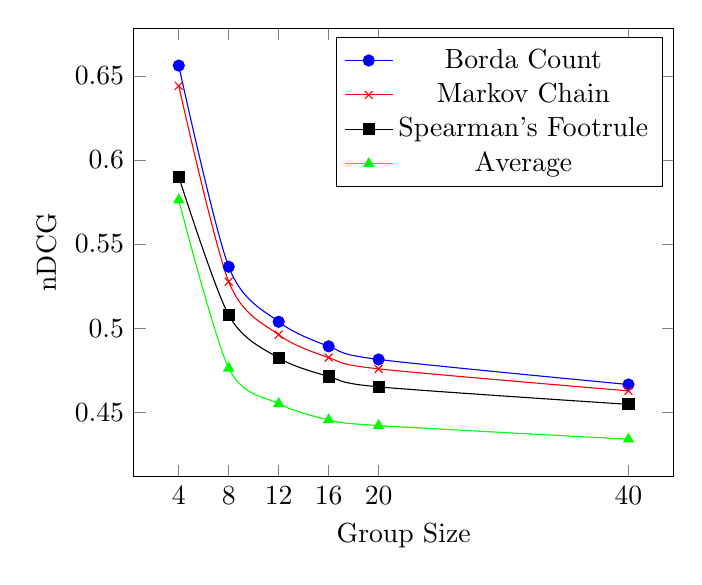
\begin{tikzpicture}
	\begin{axis}[
	xlabel=Group Size,
	ylabel=nDCG,
	xtick = {4,8,12,16,20,40}]
	\addplot[smooth,mark=*,blue] plot coordinates {
		(4,0.6561)
		(8,0.5365)
		(12,0.5038)
		(16,0.4892)
		(20,0.4814)
		(40,0.4665)
	};
	\addlegendentry{Borda Count}
	
	\addplot[smooth,color=red,mark=x] plot coordinates {
		(4,0.6440)
		(8,0.5276)
		(12,0.4961)
		(16,0.4825)
		(20,0.4758)
		(40,0.4627)
	};
	\addlegendentry{Markov Chain}
	
	\addplot[smooth,color=black,mark=square*] plot coordinates {
		(4,0.59)
		(8,0.5077)
		(12,0.4823)
		(16,0.4713)
		(20,0.4651)
		(40,0.4547)
	};
	\addlegendentry{Spearman's Footrule}
	
	\addplot[smooth,color=green,mark=triangle*] plot coordinates {
		(4,0.5762)
		(8,0.4762)
		(12,0.4551)
		(16,0.4455)
		(20,0.4421)
		(40,0.434)
	};
	\addlegendentry{Average}
	
	\end{axis}
	\end{tikzpicture}
	\caption{Results for nDCG test}\label{fig:ndcg}
\end{figure}
\subsubsection{Distance Measures}

\paragraph{Kendall Tau Distance}
\note{This is a rough draft}
Kendall tau distance is a measure of the difference between ranked lists\citep{rank:aggregation}. It counts the pairwise disagreement between two ranked lists as specified in the Equations \ref{eq:kendalldistance1}, \ref{eq:kendalldistance2} and \ref{eq:kendalldistancefinal}. The count is then normalized by dividing with $n(n-1)/2$ where $n$ is the total number of available positions, giving the maximum number of possible values. \note{check up on this}
These two equations are used when working with full lists where every list contains every item. 

\begin{equation}\label{eq:kendalldistance1}
K1(\sigma,\tau) = | \{(i,j) | i < j, \sigma (i) < \sigma (j) \land \tau (i) > \tau (j)|
\end{equation}
\begin{equation}\label{eq:kendalldistance2}
K2(\sigma,\tau) = | \{(i,j) | i < j, \sigma (i) > \sigma (j) \land \tau (i) < \tau (j) \} |
\end{equation}

\begin{equation}\label{eq:kendalldistancefinal}
K(\sigma,\tau) = k2(\sigma,\tau) + k1(\sigma,\tau)
\end{equation}

The above measure is for full lists but as we work on top-k lists we have found a modification of the standard Kendall tau distance\cite{comparing:topk}. 

 which we do by adding a third case in which it needs to count a disagreement. If a item occurs on one list but not the other it is assigned the value of the total number of items plus 1. We then add Equation \ref{eq:kendalldistance3} to Kendall tau distance in case we encounter equal items on one list which is undesirable.

\begin{equation}\label{eq:kendalldistance3}
K(\sigma,\tau) = | \{(i,j) | i < j, \sigma (i) = \sigma (j) \lor \tau (i) = \tau (j) \} |
\end{equation}

To find the distance from a recommended list to a groups preferences each list of user preferences are compared to the result list and the average distance is the result. 



\paragraph{Spearman Distance}
\section{Group Recommendation}\label{sec:grouprecommendation}
This section documents the preprocessing done and outlines the rank aggregation methods used in order make the recommendation aggregation into a group recommendation. 
%In this section we explain the workings and concept behind the four aggregation methods.

\subsection{Preprocessing}
Prior to making the rank aggregation we do some preprocessing. As specified in Figure \ref{fig:composition} the preprocessing stages get groups and all the individual recommendations as input. Preprocessing is concerned with constructing a top-k list for each of the users in a specific group based on the individual recommendations.

A top-k list is specified as a ranked list of length $k$ consisting of the highest rated items order in descending order. More specifically let $\tau$ be a top-k list and let $\tau(i)$ be the rating of item $i$, which is an arbitrary item, then list is ranked if $\tau (1) > \tau (2) > ... > \tau (k)$.

The top-k lists are stored in a array which is used as input for the aggregation methods.

\subsection{Rank Aggregation}\label{sec:aggregations}
In this section we describe the aggregation methods. Common for all the aggregation methods is that they aggregate an array of top-k lists into one ranked list, $\omega$, of length $k$ containing recommendations of a group which is returned. The order of $\omega$ may differ between the methods as they rank it based on which items they deem most relevant for the group with the most relevant item first. 

\adparagraph{Borda Count}
Aside from SF in the SFD measure, and Adjusted nDCG, BC was the best performing method.
\begin{figure}[H]
	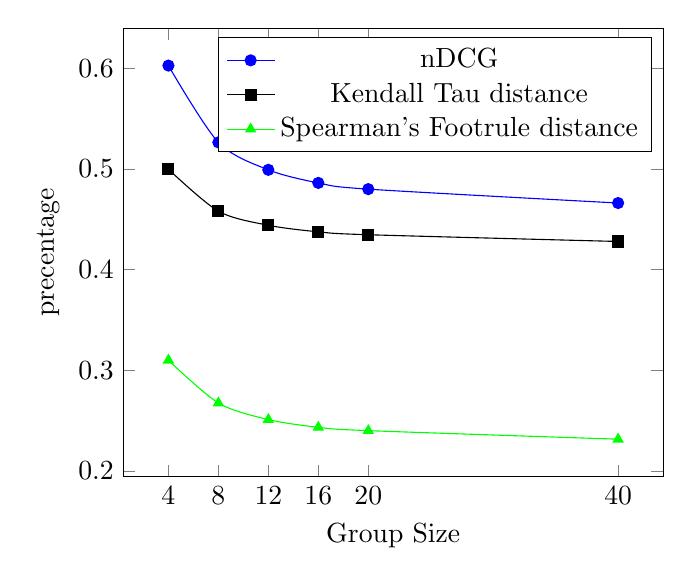
\begin{tikzpicture}
	\begin{axis}[
	xlabel=Group Size,
	ylabel=precentage,
	xtick = {4,8,12,16,20,40}]
	\addplot[smooth,mark=*,blue] plot coordinates {
		(4,0.6028)
		(8,0.5265)
		(12,0.4992)
		(16,0.4862)
		(20,0.48)
		(40,0.4662)
	};
	\addlegendentry{nDCG}
	
		\addplot[smooth,color=black,mark=square*] plot coordinates {
		(4,0.4998)
		(8,0.4581)
		(12,0.4441)
		(16,0.4376)
		(20,0.4347)
		(40,0.428)
	};
	\addlegendentry{Kendall Tau distance}
	
		\addplot[smooth,color=green,mark=triangle*] plot coordinates {
		(4,0.31)
		(8,0.2675)
		(12,0.251)
		(16,0.2433)
		(20,0.24)
		(40,0.2315)
	};
	\addlegendentry{Spearman's Footrule distance}
	
	\end{axis}
	\end{tikzpicture}
	\caption{Results for Borda Count}\label{fig:ndcganalysis}
\end{figure}

\begin{table}[H]
\centering
\label{my-label}
\begin{tabular}{|l|lllll|}\hline
     & 4 to 8 & 8 to 12 & 12 to 16 & 16 to 20 & 20 to 40 \\\hline
nDCG & 12.66  & 5.19    & 2.6      & 1.28     & 2.88     \\
KTD  & 8.34   & 3.06    & 1.46     & 0.66     & 1.54     \\
SFD  & 13.71  & 6.17    & 3.07     & 1.36     & 3.54     \\\hline
\end{tabular}
\caption{Percentage decrease between the groups for Borda Count}
\end{table}
\subsubsection{Markov Chain}\label{sec:markovchain}
%Dwork et al propose a Markov Chain for aggregating ranked lists called \MC\cite{rank:aggregation}. \MC has a set of states, $S = \{1, 2,..., |I|\}$, corresponding to a set of all the items, $I$.

Dwork et al propose a Markov Chain for aggregating ranked lists, called \MC\cite{rank:aggregation}. \MC generalizes the heuristics of the Copeland Method, where a winner is the candidate which wins the most pairwise contests\cite{saari1996}.

\MC is a process where we note the possibility of transitioning from one state to another state over time. The \MC state space, $S$, corresponds to a set of all the items, $I$, such that $S = \{1, 2,..., |I|\}$. The transition probabilities between states are represented by a transition matrix, $P = |I| \times |I|$, covering the probability, $p_{ij}$, between any item pair $i \in I$ and $j \in I$.

To calculate the probabilities, let $c_i$ be the set of items from $I$, that for the majority of the ranked lists we aggregate for, $\tau_1, \tau_2, ...,\tau_u$, it holds that $\tau_u(i) > \tau_u(j)$. The probabilities of $P$ is found according to Equation \ref{eq:markovchain_p_ij}. $\lambda$ is a variable for teleporting, which provides a small increase in accurate. Via tuning, we found that $\lambda = 0.05$ is a good value. For the case of a missing item from either or both lists, the item is considered to be on the lowest possible rank.

\begin{equation}\label{eq:markovchain_p_ij}
p_{ij} = (\frac{|c_i|}{|I|})(1-\lambda)+(\frac{\lambda}{|I|})
\end{equation}

For the probability of state $i$ staying in state $i$, we have Equation \ref{eq:markovchain_p_ii}.

\begin{equation}\label{eq:markovchain_p_ii}
p_{ii} = (\frac{|I|-|c_i|}{|I|})(1-\lambda)+(\frac{\lambda}{|I|})
\end{equation}

When the transition matrix is calculated, the result can be found via the stationary distribution for $P$. A distribution vector is a vector of size $|I|$, which holds non-negative values, representing how the states are distributed. For an initial distribution, $x$, then $xP^t$, is the same initial distribution after $t$ steps down the chain. The stationary distribution is where the state distribution stops changing regardless of taking more steps.

For practical purposes, we can approximate the stationary distribution for $P$ via application of the power-iteration algorithm. So the approximate distribution, $r$, is found in Equation \ref{eq:markovchain_power} for a number of steps, $t$. Via tuning, we found that $t = 30$ was a good value.

\begin{equation}\label{eq:markovchain_power}
r = xP^t
\end{equation}

The result of \MC is then found as the $k$ items with the biggest shares of $r$.
\subsection{Spearman's Footrule}\label{sec:spearmansfootrule}
Dwark et al also propose to use Spearman's footrule(SF) for aggregating ranked lists\citep{rank:aggregation}.
SF utilises the graph theory called bipartite graphs to construct a weighted complete bipartite graph $(S,P,W)$. 
Let $S$ be the set of items which is equal to the union of the ranked top-k lists $\tau_1, ..., \tau_k$. Then we have the set $P = \{1,...,k\}$ which is the available positions. Lastly the set $W$ is the set of edge weights between items $s\in S$ and positions $p\in P$. The weights $W(s,p)$ is found by using the scaled footrule distance equation which can be seen in equation \ref{eq:spearmanfootrule}. 
 
%$I$ is the union of users top-k lists and $P$ is the total number of positions equal to $|I|$. $E$ is the weight between an item $i \in I$ and a position $p \in P$. In Equation \ref{eq:spearmanfootrule} it is shown how the weights are calculated for full lists. 

%where the weight on the edges in $E$ is the footrule distance from note u to position v. utilises the minimum cost maximum matching method to find the best possible ranked list based on a set $L$ of ranked lists. 

\begin{equation}\label{eq:spearmanfootrule}
W(c,p) = \displaystyle\sum_{i=1}^{k} |r_i(c)/|r_i| - p/k|
\end{equation}

As we work with partial lists we will encounter lists with missing items. For this reason we have added a second case, in addition to the approach described by Dwark et al, which can be seen in Equation \ref{eq:spearmanfootruleempty}. In this case we adapt the Spearman's footrule distance variable $\ell$ which is used on partial lists. $\ell$ needs to be larger than $k$ and in our case it is $k + 1$. The reason for this is to punish infrequent items by giving them a higher weight.

\begin{equation}\label{eq:spearmanfootruleempty}
W(c,p) = \displaystyle\sum_{i=1}^{k} |(\ell/|r_i| - p/k|
\end{equation}

After determining the edge weights, the problem can be solved as a minimum cost maximum matching problem, which is the problem of finding the highest number of node matches with the lowest edge cost. To do this, we decided to use the Hungarian method\note{Or an extension called Munkres (sæt en cite)}. The result of this method is the top-k list to be recommended.
\subsection{Average}\label{sec:average}
\section{Evaluation}\label{sec:evaluation}
In this section we show our evaluation of the aggregation methods described in Section \ref{sec:aggregations}.
\chapter{Setup} \label{structure}
\section{Pipeline}	\label{st:pipeline}
The group recommender is split into different stages, 

\begin{figure}
	\centering
	
\begin{tikzpicture}
	\fill circle (1.5);
	\end{tikzpicture}
	\caption{Efficiency evaluation of near-duplicate detection on the DS1 dataset \label{fig:neardup_performance}}
\end{figure}
\section{Results}

\begin{frame}
     \begin{center}
     	\huge Results 
     \end{center}
\end{frame}

\begin{frame}
	\frametitle{Methodology}
	The setup of the new test is the same as the previous tests
	\begin{itemize}
		\item The exact same random generated groups as in the previous tests
		\item Groups of the sizes 4, 8, 12, 16, 20, and 40
		\item There are 1000 groups of each size
		\item The preferences looked at is the top 10
	\end{itemize}
\end{frame}

\begin{frame}
\frametitle{Group Size 4}
\begin{figure}[h]
\centering
\begin{minipage}{.46\textwidth}\centering
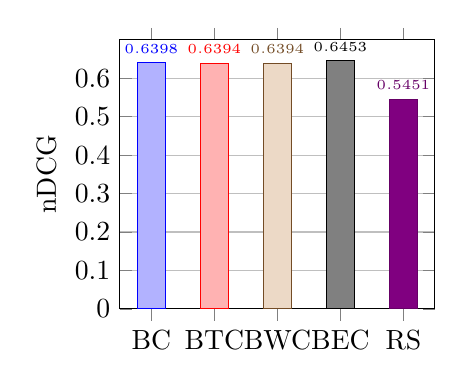
\begin{tikzpicture}
 \begin{axis}[
 	height=5cm,
 	width=4cm,
 	ybar =-10pt,
 	x = .8cm,
 	ymin=0.0, 
 	ymax=0.70,
 	ytick = {0, 0.1,0.2,0.3,...,0.70},
 	scaled y ticks = false,
	enlarge x limits ={abs=.4cm},
	nodes near coords,
    every node near coord/.append style={font=\tiny,/pgf/number format/.cd,precision=4},
 	ylabel={nDCG},
	xtick={0,1,2,3,4},  % NEW BIT
	xticklabels={BC, BTC, BWC, BEC, RS},
	%legend style={at={(0.5,-0.1)},
	%anchor=north,legend columns=-1},
	ymajorgrids = true,]

		\addplot coordinates {(0,0.6398)};    
		\addplot coordinates {(1,0.6394)};    
		\addplot coordinates {(2,0.6394)};    
		\addplot coordinates {(3,0.6453)};    
		\addplot coordinates {(4,0.5451)};
        %\legend{BC, BTC, BWC, BEC, Random}
     \end{axis}
\end{tikzpicture}
\end{minipage}
\begin{minipage}{.46\textwidth}\centering
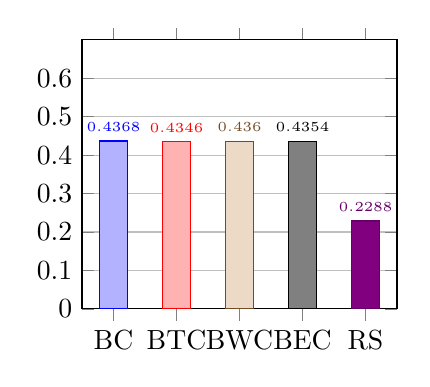
\begin{tikzpicture}
 \begin{axis}[
 	height=5cm,
 	ybar =-10pt,
 	x = .8cm,
 	ymin=0.0, 	
 	ymax=0.70,
 	ytick = {0,0.1,0.20,0.3,...,0.70},
	enlarge x limits ={abs=.4cm},
	nodes near coords,
    every node near coord/.append style={font=\tiny,/pgf/number format/.cd,precision=4},
	xtick={0,1,2,3,4},  % NEW BIT
	xticklabels={BC, BTC, BWC, BEC, RS},
	%legend style={at={(0.5,-0.1)},
	%anchor=north,legend columns=-1},
	ymajorgrids = true,]

		\addplot coordinates {(0,0.4368)};    
		\addplot coordinates {(1,0.4346)};    
		\addplot coordinates {(2,0.436)};    
		\addplot coordinates {(3,0.4354)};    
		\addplot coordinates {(4,0.2288)};
        %\legend{BC, BTC, BWC, BEC, Random}
     \end{axis}
\end{tikzpicture}
\end{minipage}
\end{figure}
\end{frame}

\begin{frame}
\frametitle{Group Size 12}
\begin{figure}[h]
\centering
\begin{minipage}{.46\textwidth}\centering
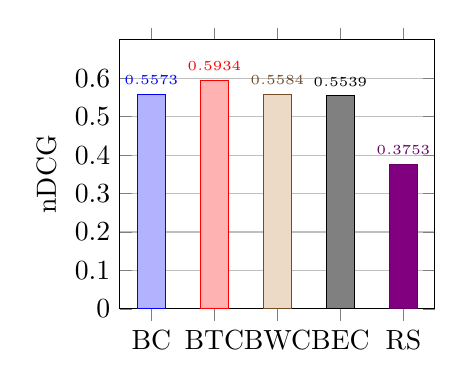
\begin{tikzpicture}
 \begin{axis}[
 	height=5cm,
 	width=4cm,
 	ybar =-10pt,
 	x = .8cm,
 	ymin=0.00, 
 	ymax=0.70,
 	ytick = {0,0.1,0.2,0.3,...,0.70},
 	scaled y ticks = false,
	enlarge x limits ={abs=.4cm},
	nodes near coords,
    every node near coord/.append style={font=\tiny,/pgf/number format/.cd,precision=4},
 	ylabel={nDCG},
	xtick={0,1,2,3,4},  % NEW BIT
	xticklabels={BC, BTC, BWC, BEC, RS},
	%legend style={at={(0.5,-0.1)},
	%anchor=north,legend columns=-1},
	ymajorgrids = true,]

		\addplot coordinates {(0,0.5573)};    
		\addplot coordinates {(1,0.5934)};    
		\addplot coordinates {(2,0.5584)};    
		\addplot coordinates {(3,0.5539)};    
		\addplot coordinates {(4,0.3753)};
        %\legend{BC, BTC, BWC, BEC, Random}
     \end{axis}
\end{tikzpicture}
\end{minipage}
\begin{minipage}{.46\textwidth}\centering
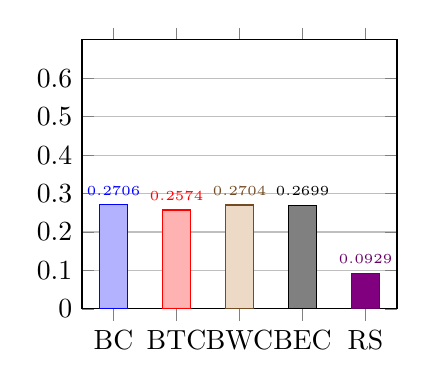
\begin{tikzpicture}
 \begin{axis}[
 	height=5cm,
 	ybar =-10pt,
 	x = .8cm,
 	ymin=0.0, 	
 	ymax=0.70,
 	ytick = {0,0.1,0.20,0.3,...,0.70},
	enlarge x limits ={abs=.4cm},
	nodes near coords,
    every node near coord/.append style={font=\tiny,/pgf/number format/.cd,precision=4},
	xtick={0,1,2,3,4},  % NEW BIT
	xticklabels={BC, BTC, BWC, BEC, RS},
	%legend style={at={(0.5,-0.1)},
	%anchor=north,legend columns=-1},
	ymajorgrids = true,]

		\addplot coordinates {(0,0.2706)};    
		\addplot coordinates {(1,0.2574)};    
		\addplot coordinates {(2,0.2704)};    
		\addplot coordinates {(3,0.2699)};    
		\addplot coordinates {(4,0.0929)};
        %\legend{BC, BTC, BWC, BEC, Random}
     \end{axis}
\end{tikzpicture}
\end{minipage}
\end{figure}
\end{frame}

\begin{frame}
\frametitle{Group Size 40}
\begin{figure}[h]
\centering
\begin{minipage}{.46\textwidth}\centering
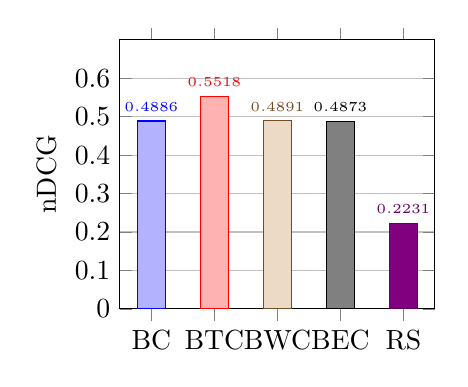
\begin{tikzpicture}
 \begin{axis}[
 	height=5cm,
 	width=4cm,
 	ybar =-10pt,
 	x = .8cm,
 	ymin=0.00, 
 	ymax=0.70,
 	ytick = {0,0.1,0.20,0.3,0.4,0.5,0.60},
 	scaled y ticks = false,
	enlarge x limits ={abs=.4cm},
	nodes near coords,
    every node near coord/.append style={font=\tiny,/pgf/number format/.cd,precision=4},
 	ylabel={nDCG},
	xtick={0,1,2,3,4},  % NEW BIT
	xticklabels={BC, BTC, BWC, BEC, RS},
	%legend style={at={(0.5,-0.1)},
	%anchor=north,legend columns=-1},
	ymajorgrids = true,]

		\addplot coordinates {(0,0.4886)};    
		\addplot coordinates {(1,0.5518)};    
		\addplot coordinates {(2,0.4891)};    
		\addplot coordinates {(3,0.4873)};    
		\addplot coordinates {(4,0.2231)};
        %\legend{BC, BTC, BWC, BEC, Random}
     \end{axis}
\end{tikzpicture}
\end{minipage}
\begin{minipage}{.46\textwidth}\centering
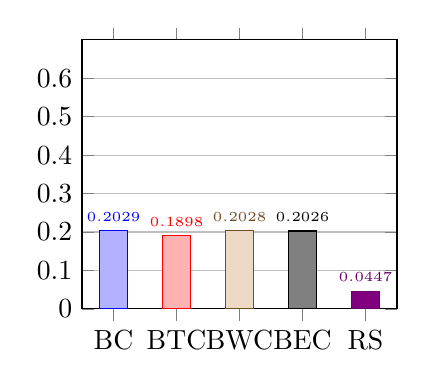
\begin{tikzpicture}
 \begin{axis}[
 	height=5cm,
 	ybar =-10pt,
 	x = .8cm,
 	ymin=0.0, 	
 	ymax=0.70,
 	ytick = {0,0.1,0.20,0.3,0.4,0.5,0.60},
	enlarge x limits ={abs=.4cm},
	nodes near coords,
    every node near coord/.append style={font=\tiny,/pgf/number format/.cd,precision=4},
	xtick={0,1,2,3,4},  % NEW BIT
	xticklabels={BC, BTC, BWC, BEC, RS},
	%legend style={at={(0.5,-0.1)},
	%anchor=north,legend columns=-1},
	ymajorgrids = true,]

		\addplot coordinates {(0,0.2029)};    
		\addplot coordinates {(1,0.1898)};    
		\addplot coordinates {(2,0.2028)};    
		\addplot coordinates {(3,0.2026)};    
		\addplot coordinates {(4,0.0447)};
        %\legend{BC, BTC, BWC, BEC, Random}
     \end{axis}
\end{tikzpicture}
\end{minipage}
\end{figure}
\end{frame}

\begin{frame}
	\frametitle{Possible Solutions}
	\begin{itemize}
		\item Calculate nDCG using the predicted ratings
		\item Ordering the individual ranked list by the average for the group
	\end{itemize}
\end{frame}
\section{Discussion} \label{sec:discussion}
Across all the methods tested we saw a similar fall in nDCG scores and distance for the distance measures as group size increased, except for some methods in Rating nDCG.

We also saw a trend of the nDCG score being a good indicator for how well the same  methods performed for the distance measure. Though SF performed well in SFD, but it fell behind on other measures, with the same to be said for Avg and its performance for Rating nDCG. This stresses the importance of testing a general purpose method from many angles.

Across all the measurements, \MC is almost identical in performance to that of BC. As the underlying heuristic of the \MC method is the Copeland Method, it raises the possibility that other extensions of Markov Chain can achieve even greater results.

However, for \MC, other factors such as complexity and speed limits the utility of it compared to BC, as BC is both simple to implement and can be implemented in linear time whereas \MC is usually slower and our implementation reflected this. However optimizations for \MC and its variants exists which run in quadratic time which is a significant running time improvement\cite{rank:aggregation}.

Of all the measures, Avg has the worst results overall aside from Rating nDCG. The results from Rating nDCG in isolation sees Avg perform the best. So if Rating nDCG is a better measurement because it does not consider the rankings, and instead looks directly at the ratings given by the users, then Avg is providing the better recommendations.

However, results from Rating nDCG for Avg and the other methods are so close that there is little practical value for one method to the other. Should it be the case that Rating nDCG is the best measure, we have a theory about rearranging the users top-k list and order them according to average. We will expand on this in future work in Section \ref{sec:futurework}.

Baltrunas et al found that the more alike a group is, the more effective the group recommender\cite{Baltrunas:2010:GRR:1864708.1864733}. Likewise for our setup, it is likely that the results can vary depending on the recommender used in the individual recommendations stage. It follows that biases introduced by the individual recommendation can result in an either more or less alike-thinking group for the same dataset.

%All methods saw similar decreases in effectiveness across group sizes.

%BC performed best for nDCG. Other benefits include fast computation time, simple to implement. Outperforms or stands equal to various extensions we've developed. Compared with MC for nDCG, the mean difference is small, but consistent.

%MC performed 2nd best for nDCG. Our implementation is very slow, but it can be optimized a lot (probably still not faster than BC). No indication in data, but might surprise for bigger topK lists, which in turn raises the connectivity (main strength). Runs on the Copeland method, which is ill regarded for aggregation, but works reasonably well here.

%Avg generally performs poorly. It gets some good results in Adjusted nDCG, but that is a measurement uniquely advantageous for it among the methods, so it makes little sense as a measure.

%X method is the best

%When to use kendall and nDCG? For our results, it's not that important.
\chapter{Conclusion} \label{ch:conclusion}
We wanted to showcase an approach that reconciles the differences in preferences among multiple group members in the problem of group recommendation. During this process we found that the evaluation possibilities of the performance of these approaches were rather limited due to lack of proper datasets making it difficult to determine whether or not a group would be satisfied with its recommendations.

We found that with using a ranked list for the recommendations we could adopt the normalized Discounted Cumulative Gain(nDCG) technique from the information retrieval domain to measure user satisfaction by comparing the ranked list of a user with the ranked list found through aggregation. This only left us with the task of forming the groups, which we ended up doing using random sampling.

We sought to answer the following questions from the problem statement:
\begin{itemize}
	\item How to reflect group decision making algorithmically while securing satisfaction for the individuals as well as the group as a whole?
	\item How to measure the level of satisfaction in a group in regards to the items recommended?
	\item How to make recommendations to a group of people based on the users' individual preferences?
\end{itemize}

For reflecting how a group decision would be handled, we ventured into some of the methods used for resolving differing opinions. In the end, we incorporated single transferable vote into the Borda Count method in the Borda Transferable Count(BTC) algorithm. These are not methods that necessarily reflects an organic group decision process, but reflects parts of real group decision methodologies.

For measuring the level of satisfaction in a group, we found and used nDCG. It is commonly used for rankings and information retrieval. This works well with the view of recommendation as a tool for drawing out relevant information, when getting an overview is hard.

For making recommendations to a group, we present the BTC as a method of aggregating the individual ranked lists. The results are promising, as it performs better than the tested methods on nDCG scores. However, we cannot as of yet make a definite conclusion on the BTC as a solution to the group recommender problem.
\clearpage
\section{Discussion}\label{sec:conclusion_discussion}
As mentioned we use the information retrieval method nDCG to measure satisfaction. In doing so we make several assumptions about the users’ preferences. First of all, the user ratings used for the group recommendations are predictions, which may not coincide with the actual preferences of the user. Based on these predicted ratings we assume that a user would construct a ranked list, with a fixed distance between the top ranked and next highest rank regardless of the predicted preference for either, which we use to determine the satisfaction score, with the highest ratings. This means that the satisfaction score we get is based on assumptions about a user's preferences, which makes our results noteworthy, but ultimately, based on assumptions about existing data rather than real world data.

In order for us to get a concrete result we need to measure satisfaction with real users as to prove the effectiveness of the method presented in this project. Provided that, the method could point in the direction that group recommendation is a voting problem.

\bibliographystyle{ACM-Reference-Format}
\bibliography{references} 

\begin{appendices}
\section{Survey}
%Context about why we needed the data

%How the whole thing went down
In order to make a dataset in a short time frame, we looked into crowdsourcing, where it was possible to pay people to answer surveys or do tasks that computers cannot. In particular we were looking at Clickworker and Mechanical Turk, which allowed external surveys. Since no sites had an inbuilt survey creation tool that could handle our requirements, we decided to make our own survey website.

Using this method, we could potentially reach thousands of people without limiting us to the survey tools made available on the standard websites.

%Creation of the website
For web hosting, we went to DigitalOcean, which offered a Ubuntu server setup with Django. We added Gunicorn as the WSG interface and nginx as the http server. Behind it all, we had a MySql database keeping track of the survey questions and results along with timestamps.

%Django as Python web application framework
%Gunicorn as Web Server Gateway Interface(WSGI) server. A traditional web server does not understand or have any way to run Python applications. WSGI is a standard interface for py modules and containers.
%Digical Ocean as webhost with Unix as the OS
%MySql as the database

%The survey
The survey itself asks participants to personally give a recommendation to a group of users. The participant knows each user's own top 10 preference, and must decide on their own what aggregation strategy they wish to follow. An important aspect of the survey was making it as easy to complete as possible. As we had to pay each participant, each such improvement could be translated to a saving, which in turn translated to a larger and more useful dataset. So to make it more intuitive and not overload each user with information, we made it so that hovering the mouse over a movie title will make the movie's position light up on all the other users' rankings, shown in Figure \ref{fig:appendix_userprefs}, and gave the user a tooltip about other movie positions. Additionally, we made the ranking system into a drag-and-drop, such that the participant could drag and easily rearrange their recommendations. This can be seen in Figure \ref{fig:appendix_recbox}.

\begin{figure}
	\includegraphics[scale=0.35]{graphics/recbox.png}
	\caption{The list of available items and the box holding the recommendations of the survey participant}
	\label{fig:appendix_recbox}
\end{figure}

\begin{figure}
	\includegraphics[scale=0.5]{graphics/users.png}
	\caption{Two lists of movie preferences for a user}
	\label{fig:appendix_userprefs}
\end{figure}

After making a recommendation, the user could proceed to the next step, and upon completing all steps they would reach a screen providing them with a code. With each step, the group size is increased by one, going from 4 to 8 users. The code is important, as the participant must present this as evidence to the crowdsourcing site as proof of their participation. For our survey, we decided to generate a unique code for each participant mixing the assigned groups and a timestamp, so that we could deduce which user responded when and with what. This precaution was necessary so that it was possible to filter out participants rushing through the survey with no care for their answers.

Also, since we wanted to have a balanced dataset, we separated our groups into 40 sets of groups of size 4 to 8, and made it so that every user would get a randomly picked set. The database would keep track of how many responses each set had, such that we could prioritize the sets with fewer responses and get a balanced dataset. It would also mean that anyone taking the test twice would be unlikely to see the same survey.

Before running the survey on Mechanical Turk, we ran it past some other willing participants for evaluation and decided to halve the number of groups each participants would give recommendations to from 10 to 5, due to feedback about the length of the survey.

%Most importantly, we realized how vital it was to make the par

%Dealing with mechanical turk
For the crowdsourcing website, we ended up going with Amazon's Mechanical Turk, as it is the more well-known and cheaper service. When ready, we injected a good amount of money on the account, as one had to prepay for any work requested and started up a limited run to test out the services and find a suitable price range. We managed to get a few responses. On Mechanical Turk, the participant would see our survey, click in and be provided a link to our survey. Upon completion of the survey, our participant would get the code and input it on the Mechanical Turk website. Initial results were interesting with big differences between how much time participants spent on the survey. We noted a few obvious cheaters who blazed through a survey in seconds thanks to the timestamps, however as a requester and with the timestamps in our database, we would be able to sort them out, and we could also reject their work on the Mechanical Turk site.

Though, on the third day of this limited run we ran into problems with Amazon Mechanical Turk. We were unable to access our account, and had to contact their support team. Soon enough the support team responded that our account had been suspended, and that we would be informed about the reason for the suspension in 2-3 days along with fate of our account. In two days time, Mechanical Turk support wrote us that our account had been suspended indefinitely and our current survey stopped because of a violation of the participation agreement. Unaware of any possible violations we could have made, we made further inquires, but never got a clear answer. Additionally, our funds on the account were also confiscated. So in the end, we ended up only getting responses totaling a few dollars worth of data.

%Show data and evaluate on them.
\end{appendices}

\end{document}
